\documentclass[a4paper]{article}
\usepackage[T1]{fontenc}
\usepackage[russian]{babel}
\usepackage[pdftex]{graphicx}
\usepackage[ruled,vlined]{algorithm2e}
\usepackage[utf8]{inputenc}
\usepackage{xcolor}
\usepackage{hyperref}
\usepackage{amsmath}
\usepackage{geometry}
\usepackage{float}
\usepackage{caption}
\usepackage{subcaption}
\DeclareGraphicsExtensions{.pdf,.png,.jpg}

\begin{document}

    \begin{titlepage}
        \Large
        \begin{center}
            Санкт-Петербургский \ Политехнический университет Петра Великого\\
            \vspace{10em}Отчет по лабораторной работе №1\\
            \vspace{2em}
            \textbf{Изучение характеристик распределений}
        \end{center}
        \vspace{6em}
        \hfill\parbox{10cm}{
            \hspace*{2cm}\hspace*{-4cm}Студент:\hfill Швачко Никита Андреевич\\
            \hspace*{2cm}\hspace*{-4cm}Преподаватель:\hfill Баженов Александр Николаевич\\
            \hspace*{2cm}\hspace*{-4cm}Группа:\hfill 5030102/20202
        }
        \vspace{\fill}
        \begin{center}
            Санкт-Петербург \ 2025
        \end{center}
    \end{titlepage}


    \section{Формулировка задания и его формализация}\label{sec:----2}
    Для 4 распределений:
    \\- Нормальное распределение $N(x, 0,1)$
    \\- Распределение Коши $C(x, 0,1)$
    \\- Распределение Пуассона $P(k, 10)$
    \\- Равномерное распределение $U(x,-\sqrt{3}, \sqrt{3})$
    \\1. Сгенерировать выборки размером 10,50 и 1000 элементов. Построить на одном рисунке гистограмму и график плотности распределения.
    \\2. Сгенерировать выборки размером 10,100 и 1000 элементов. Для каждой выборки вычислить следующие статистические характеристики положения данных:
    $\bar{x}, \operatorname{med} x, z_Q$. Повторить такие вычисления 1000 раз для каждой выборки и найти среднее характеристик положения и их квадратов:

    $$
    E(z)=\bar{z}
    $$


    \\  Вычислить оценку дисперсии по формуле:

    $$
    D(z)=\overline{z^2}-\bar{z}^2
    $$


    Представить полученные данные в виде таблиц.
    \\ Пояснение

    $$
    z_Q=\frac{z_{1 / 4}+z_{3 / 4}}{2}
    $$


    \section{Гистограммы и графики плотности распределений}\label{sec:----}
    \begin{figure}[H]
        \centering
        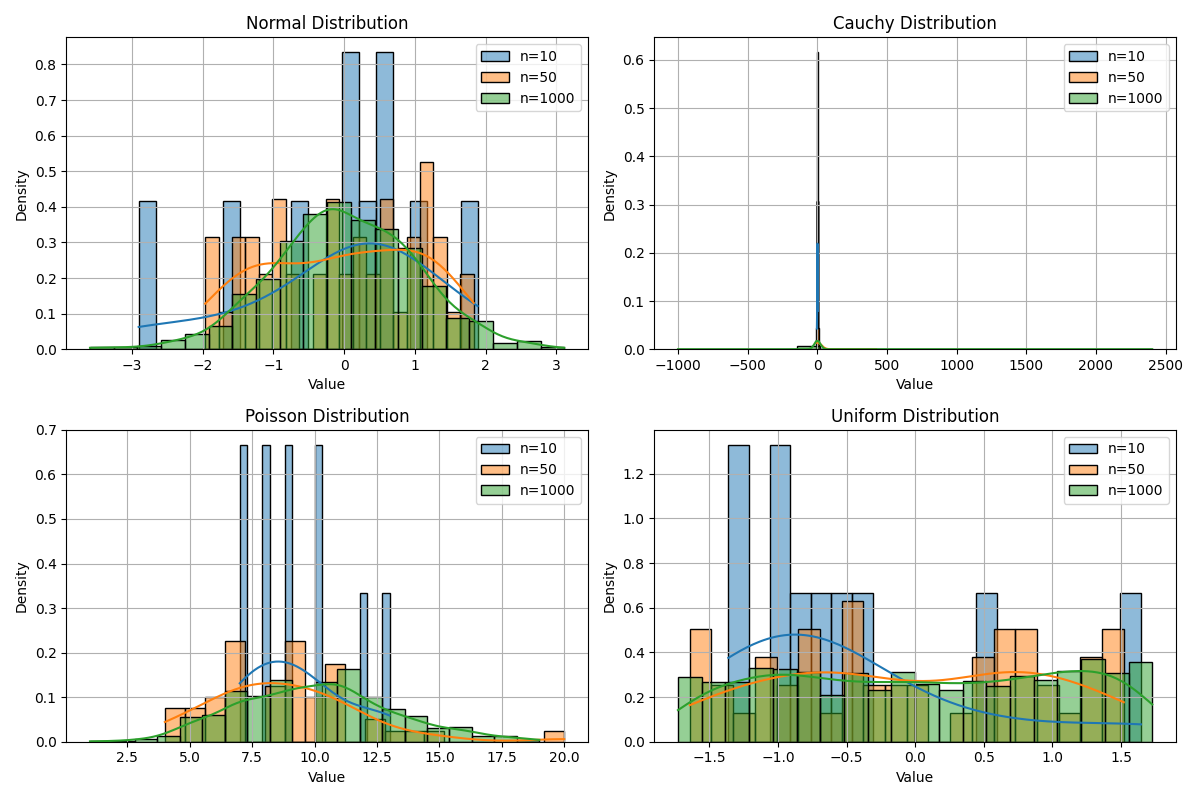
\includegraphics[width=1\textwidth]{../histograms} % Вставить график
        \caption{Гистограммы и плотности распределений для выборок разного размера}\label{fig:figure}
    \end{figure}

\newpage
    \section{Результаты вычислений статистических характеристик}\label{sec:---}
    \begin{table}[!htbp]
        \centering
        \caption{Средние значения характеристик положения и их дисперсии}

\scalebox{0.8}{



        \begin{tabular}{|c|c|c|c|}
            \multicolumn{1}{|c|}{\textbf{Нормальное}} \\
            \hline
            \textbf{Выборка} & \textbf{Характеристика} & \textbf{E(z)} & \textbf{D(z)} \\
            \hline
            10               & $\bar{x}$               & -0.014989     & 0.093232      \\
            10               & $\operatorname{med} x$  & -0.007998     & 0.132113      \\
            10               & $z_Q$                   & -0.012284     & 0.104357      \\            \hline

            100              & $\bar{x}$               & -0.001765     & 0.009737      \\
            100              & $\operatorname{med} x$  & -0.001570     & 0.015596      \\
            100              & $z_Q$                   & -0.001640     & 0.012310      \\            \hline

            1000             & $\bar{x}$               & -0.000572     & 0.001076      \\
            1000             & $\operatorname{med} x$  & 0.000240      & 0.001581      \\
            1000             & $z_Q$                   & 0.000158      & 0.001267      \\
            \hline \\
            \multicolumn{1}{|c|}{\textbf{Коши}} \\
            \hline
            \textbf{Выборка} & \textbf{Характеристика} & \textbf{E(z)} & \textbf{D(z)} \\
            \hline
            10               & $\bar{x}$               & -1.505235     & 1108.105054   \\
            10               & $\operatorname{med} x$  & -0.017018     & 0.302457      \\
            10               & $z_Q$                   & -0.012012     & 1.031296      \\            \hline

            100              & $\bar{x}$               & 0.495179      & 588.956098    \\
            100              & $\operatorname{med} x$  & -0.004341     & 0.023064      \\
            100              & $z_Q$                   & -0.001379     & 0.047650      \\            \hline

            1000             & $\bar{x}$               & -4.693015     & 15138.951738  \\
            1000             & $\operatorname{med} x$  & 0.003096      & 0.002698      \\
            1000             & $z_Q$                   & 0.001666      & 0.004582      \\
            \hline \\
            \multicolumn{1}{|c|}{\textbf{Пуассон}} \\
            \hline
            \textbf{Выборка} & \textbf{Характеристика} & \textbf{E(z)} & \textbf{D(z)} \\
            \hline
            10               & $\bar{x}$               & 10.053200     & 0.972590      \\
            10               & $\operatorname{med} x$  & 9.907000      & 1.334851      \\
            10               & $z_Q$                   & 9.981000      & 1.121795      \\            \hline

            100              & $\bar{x}$               & 9.993180      & 0.106959      \\
            100              & $\operatorname{med} x$  & 9.821500      & 0.231888      \\
            100              & $z_Q$                   & 9.911000      & 0.152048      \\            \hline

            1000             & $\bar{x}$               & 10.005329     & 0.009714      \\
            1000             & $\operatorname{med} x$  & 9.995500      & 0.004230      \\
            1000             & $z_Q$                   & 9.995750      & 0.002544      \\
            \hline \\
            \multicolumn{1}{|c|}{\textbf{Равномерное}} \\
            \hline
            \textbf{Выборка} & \textbf{Характеристика} & \textbf{E(z)} & \textbf{D(z)} \\
            \hline
            10               & $\bar{x}$               & 0.010461      & 0.101281      \\
            10               & $\operatorname{med} x$  & 0.022253      & 0.230328      \\
            10               & $z_Q$                   & 0.005793      & 0.142707      \\            \hline

            100              & $\bar{x}$               & -0.001042     & 0.009808      \\
            100              & $\operatorname{med} x$  & -0.003123     & 0.027535      \\
            100              & $z_Q$                   & 0.000367      & 0.014908      \\            \hline

            1000             & $\bar{x}$               & -0.000448     & 0.001014      \\
            1000             & $\operatorname{med} x$  & -0.001100     & 0.002945      \\
            1000             & $z_Q$                   & -0.000583     & 0.001484      \\
            \hline
        \end{tabular}
}
        \label{tab:table}
    \end{table}


    \section{Выводы}\label{sec:}
    \begin{itemize}
        \item При увеличении размера выборки характеристики положения стабилизируются.
        \item Среднее значение $\bar{x}$ для распределения Коши не является надежным из-за сильных выбросов.
        \item Медиана и квартильный средний $z_Q$ показывают меньшую изменчивость в выборках с выбросами.
        \item Пуассоновское распределение при больших $n$ приближается к нормальному.
        \item Равномерное распределение демонстрирует низкую изменчивость статистик.
    \end{itemize}


\end{document}
